\chapter{Ergebnisse dieser Arbeit}

\section{Beschreibung und Funktionalität des Prototyps}

Was kann der Prototyp?
Für was dient es?

\section{Zusammenfassung der Ergebnisse}

\subsection{Kalkulationsergebnisse}

Gesamtkosten anzeigen

\subsection{Messungsergebnisse}

In diesem Abschnitt werden die Messungsergebnisse der Performance Messung bereitgestellt. Die Speicherklassen Standard, Standard-IA und One Zone-IA von AWS wurden jeweils mit Standard, Nearline und Coldline von GC verglichen. Im folgenden werden die Ergebnisse der Upload Geschwindigkeit aller Speicherklassen als Liniendiagramm dargestellt:

\begin{figure}[h]
	\centering
	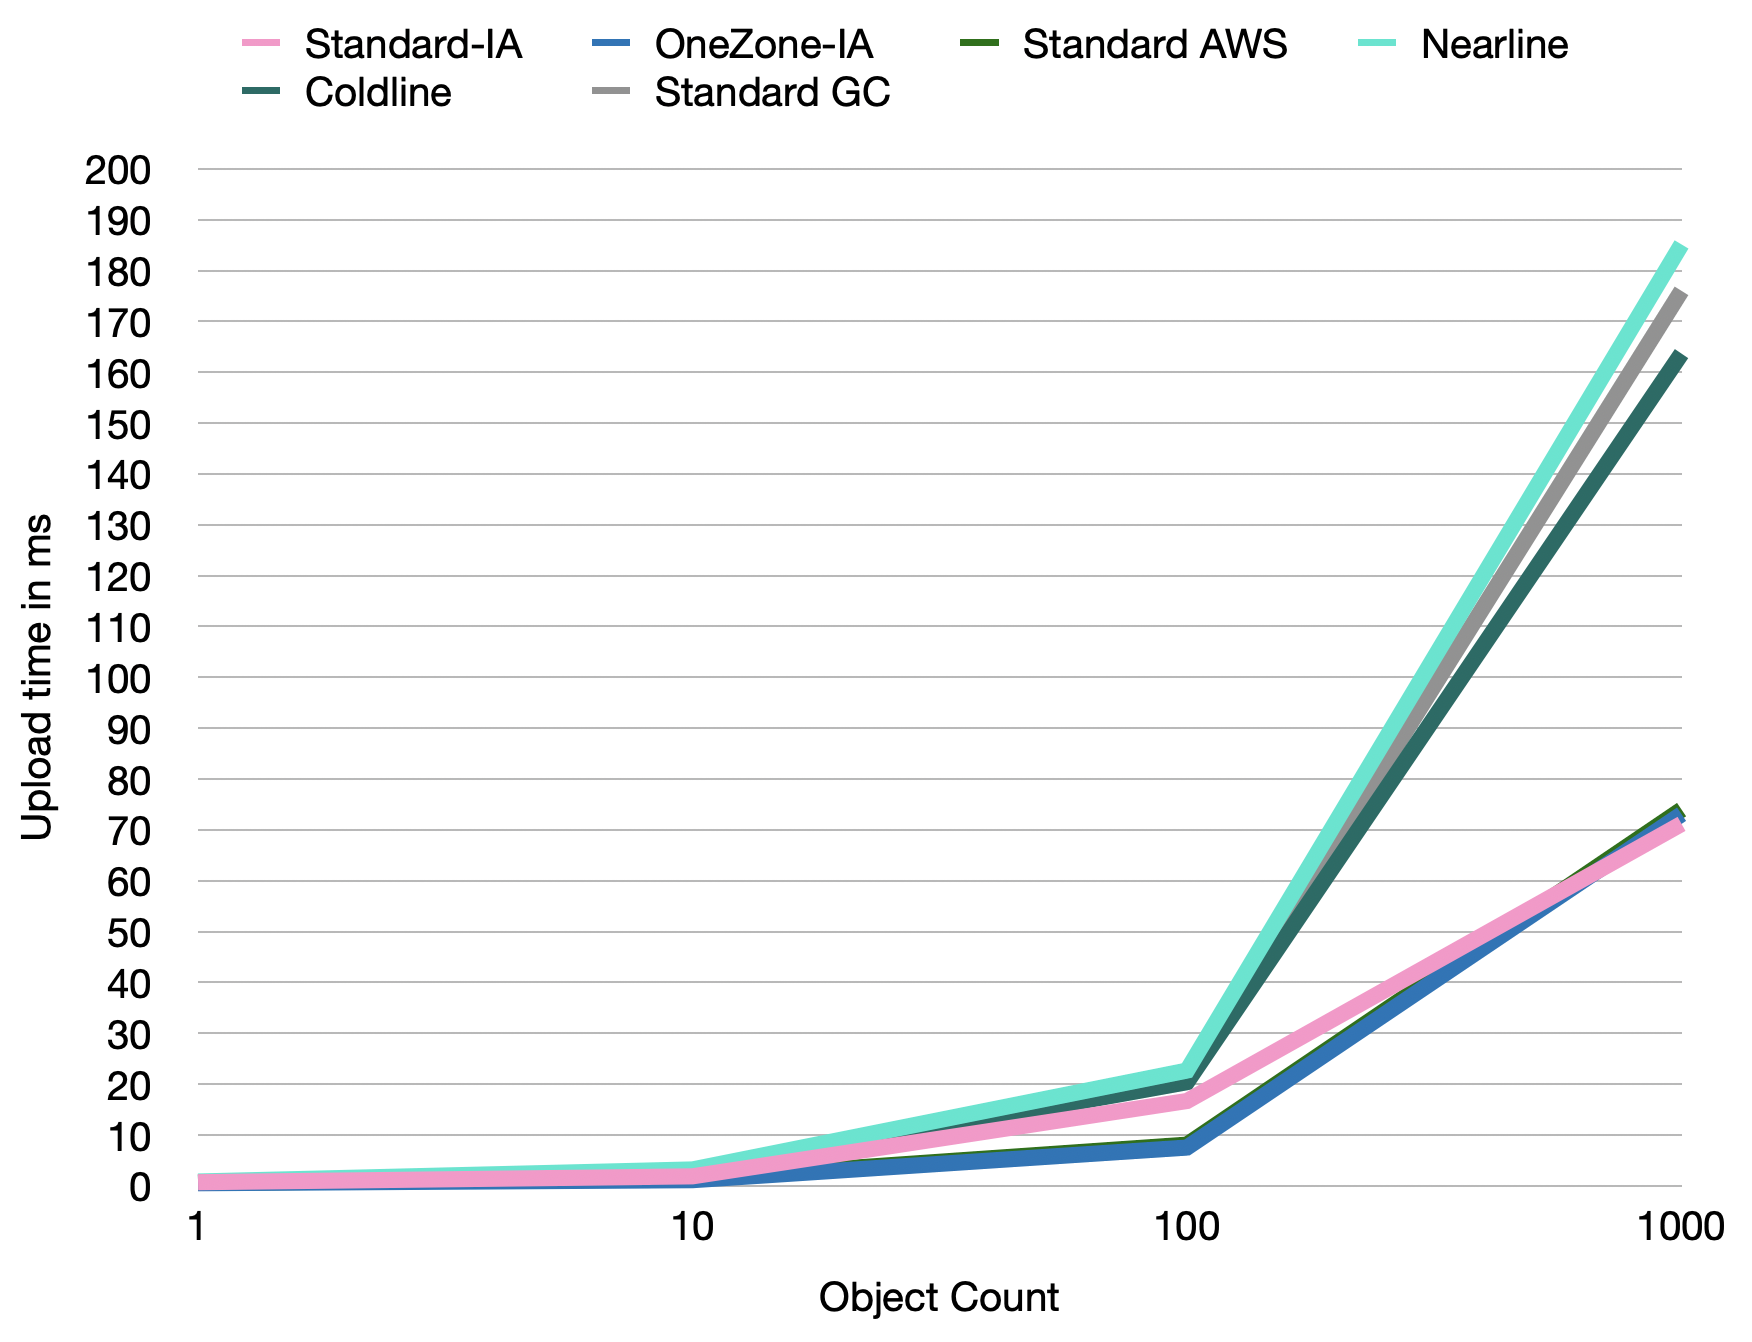
\includegraphics[width=13cm,keepaspectratio]{Pictures/UploadTime.png}
	\caption{Liniendiagramm - Upload Zeit der verschiedenen Speicherklassen}
\end{figure}	

In der obigen Abbildung wird die Upload Geschwindigkeit in Millisekunden auf der Y-Achse beschrieben. Die X-Achse beschreibt die Objektanzahl, die für jede Speicherklasse hochgeladen wurde. Die Farben unterscheiden die verschiedenen Speicherklassen voneinander, wobei die Speicherklassen von AWS jeweils nebeneinander platziert sind, genauso wie für die Speicherklassen von GC.

\begin{figure}[h]
	\centering
	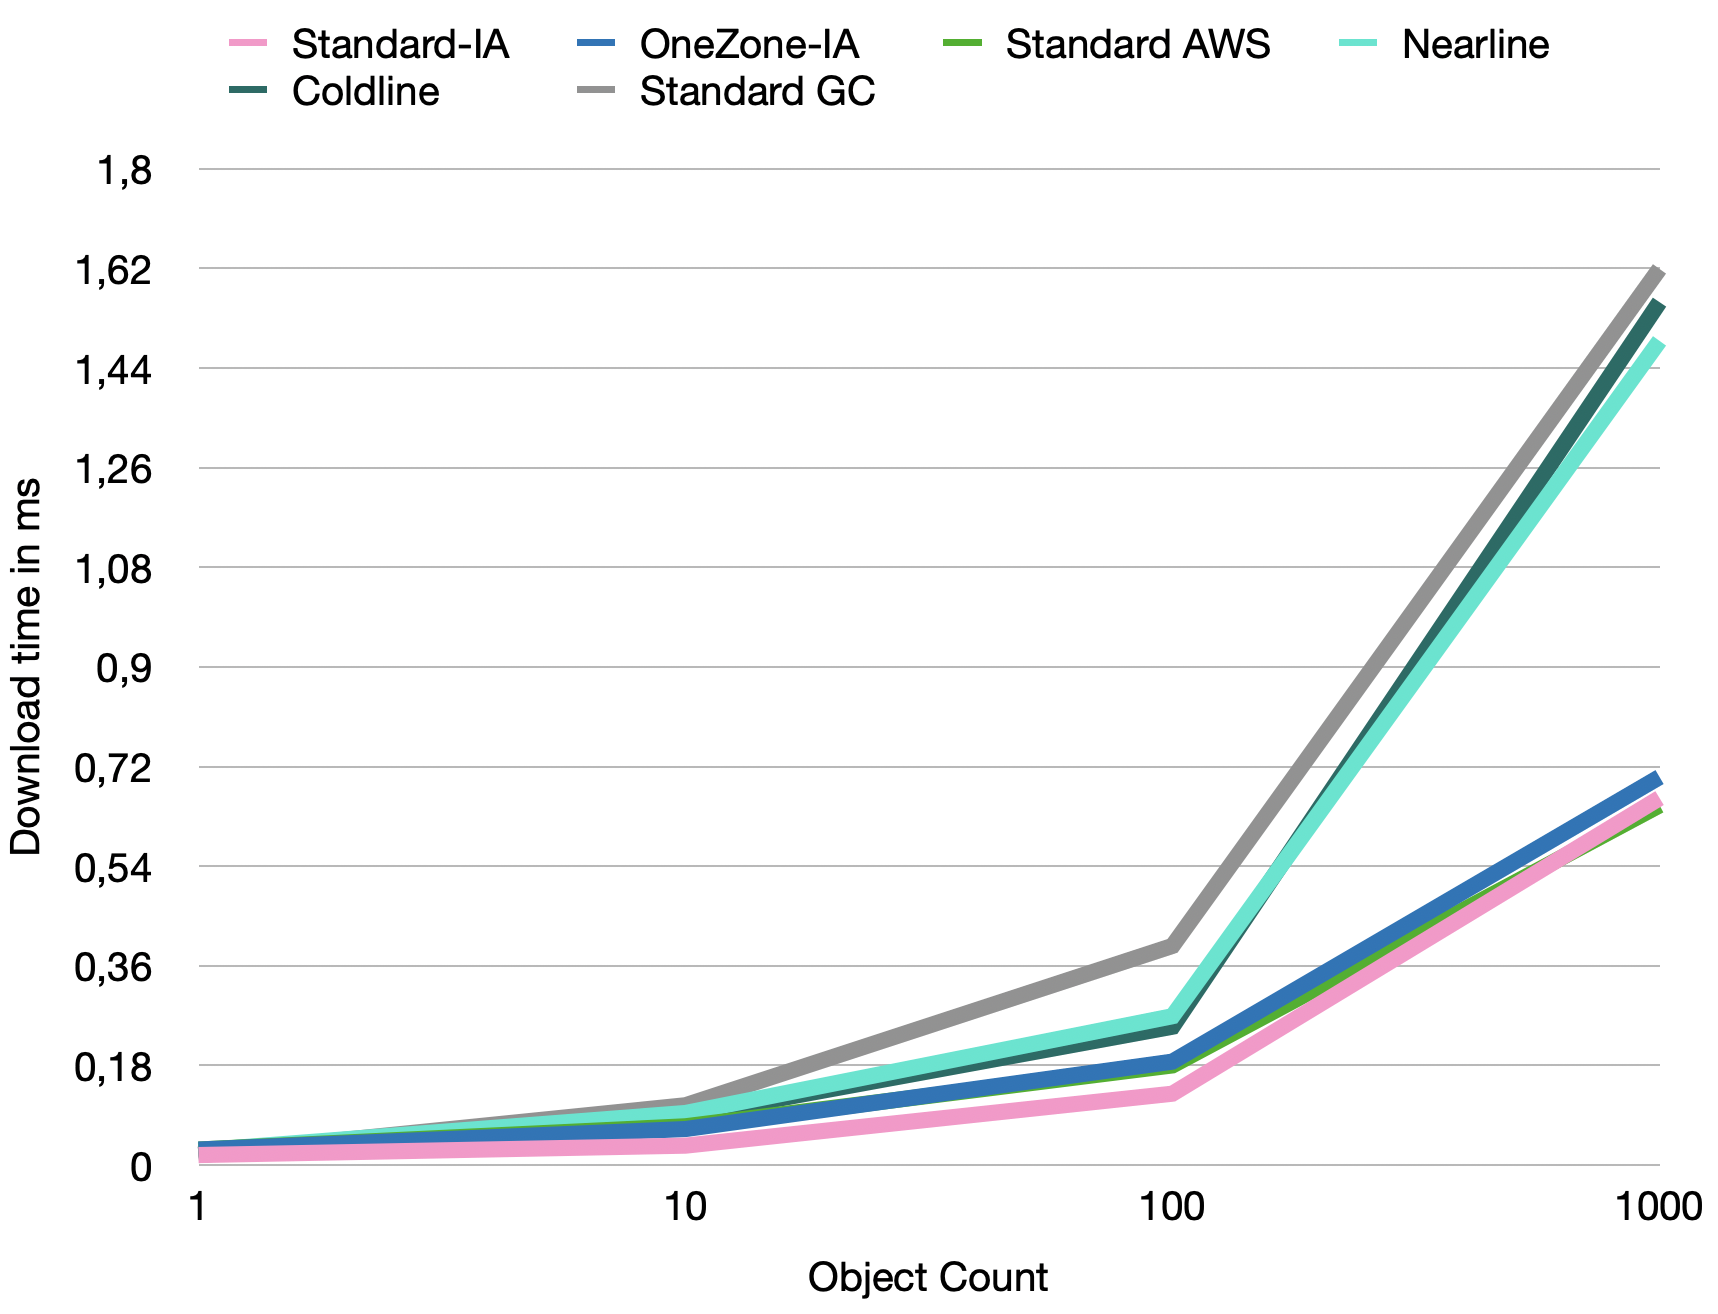
\includegraphics[width=13cm,keepaspectratio]{Pictures/DownloadTime.png}
	\caption{Lininediagramm - Download Zeit der verschiedenen Speicherklassen}
\end{figure}

Die Ergebnisse ergeben, dass AWS im Durchschnitt Dateien schneller hoch-, und heruntergeladen hat. 